\section{Algorithm Comparison}\label{sec:reconalgcomp}
From a surface reconstruction perspective, the point clouds generated from our light ring model have a number of important characteristics. The only data outputted by stereo matching is the (x,y,z) coordinates of the image points in space with respect to their relative camera poses. These points can additionally coincide with RGB values from the image, but due to the nature of our data collected the colors are always some of the highest intensity pixel values and thus much of the texture detail is lost. Because no other data is currently saved with the point data, we lack information about the point normals. At the same time, there are often outlier points that make it to the stereo matching phase. One advantage of our method is that since we only project points on the ring of light which should be in a different location every frame, theoretically our points should have limited overlap. With these problem specifics and constraints defined, the task now becomes identifying a proper surface reconstruction technique to form our initial base mesh.

For the sake of rapid prototyping different reconstruction methods on our data set, tests were run using the application Meshlab. Meshalb has a number of the techniques discussed in \ref{sec:reconrelwork} built in making it a quick option for comparing the outputs. Tests run in Meshlab could not be integrated into our pipeline, but they helped identify the proper procedure. 

Our pipeline renders our point cloud using the Point Cloud Library(PCL). PCL has a number of additional functionalities that can help in the reconstruction phase. First off, statistical outlier removal can be applied to our points. Mean distances are computer for each point in regards to its neighboring points. Points whose mean distances exceed that of the global mean and standard deviation are labeled outliers and removed from the set. This eliminates points that were picked up by the feature detector in  the image processing stage, but whos spacial position would only distort the final reconstruction. Second, we can apply the normal calculation and orientation described in \ref{sec:reconrelwork}. The points we projected from the image are all on the inside of the cave, so all of the normals should be oriented inwards. PCL makes the assumption that normals are oriented towards the camera, which is exactly what we want since our camera moves through the inside of the cave. A subset of the resulting normals can be seen in \ref{fig:showing_normals}.

\begin{figure*}[ht]
	\begin{center}
		\leavevmode
		\begin{tabular}{cc}
			\subfloat[]{{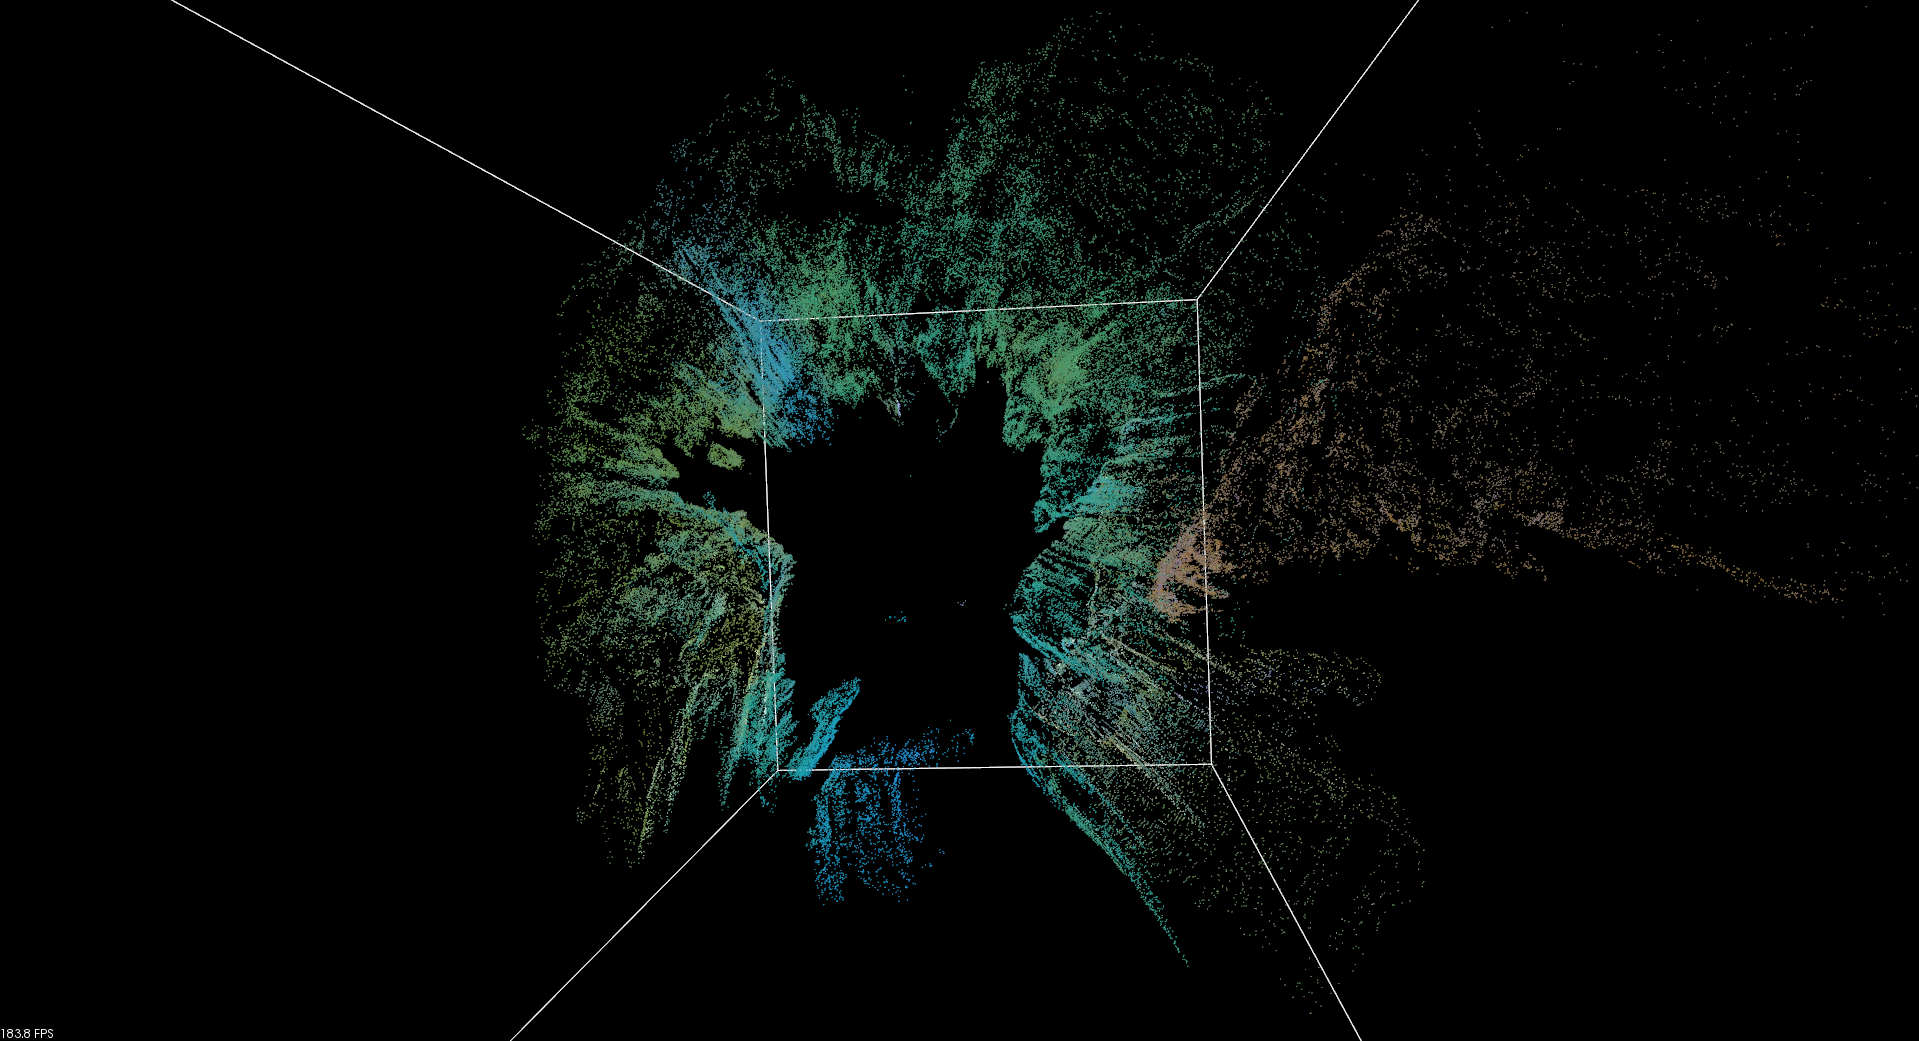
\includegraphics[width=0.95\textwidth]{./figures/normals_pcl_without}\label{fig:without_normals}}}\\
			\subfloat[]{{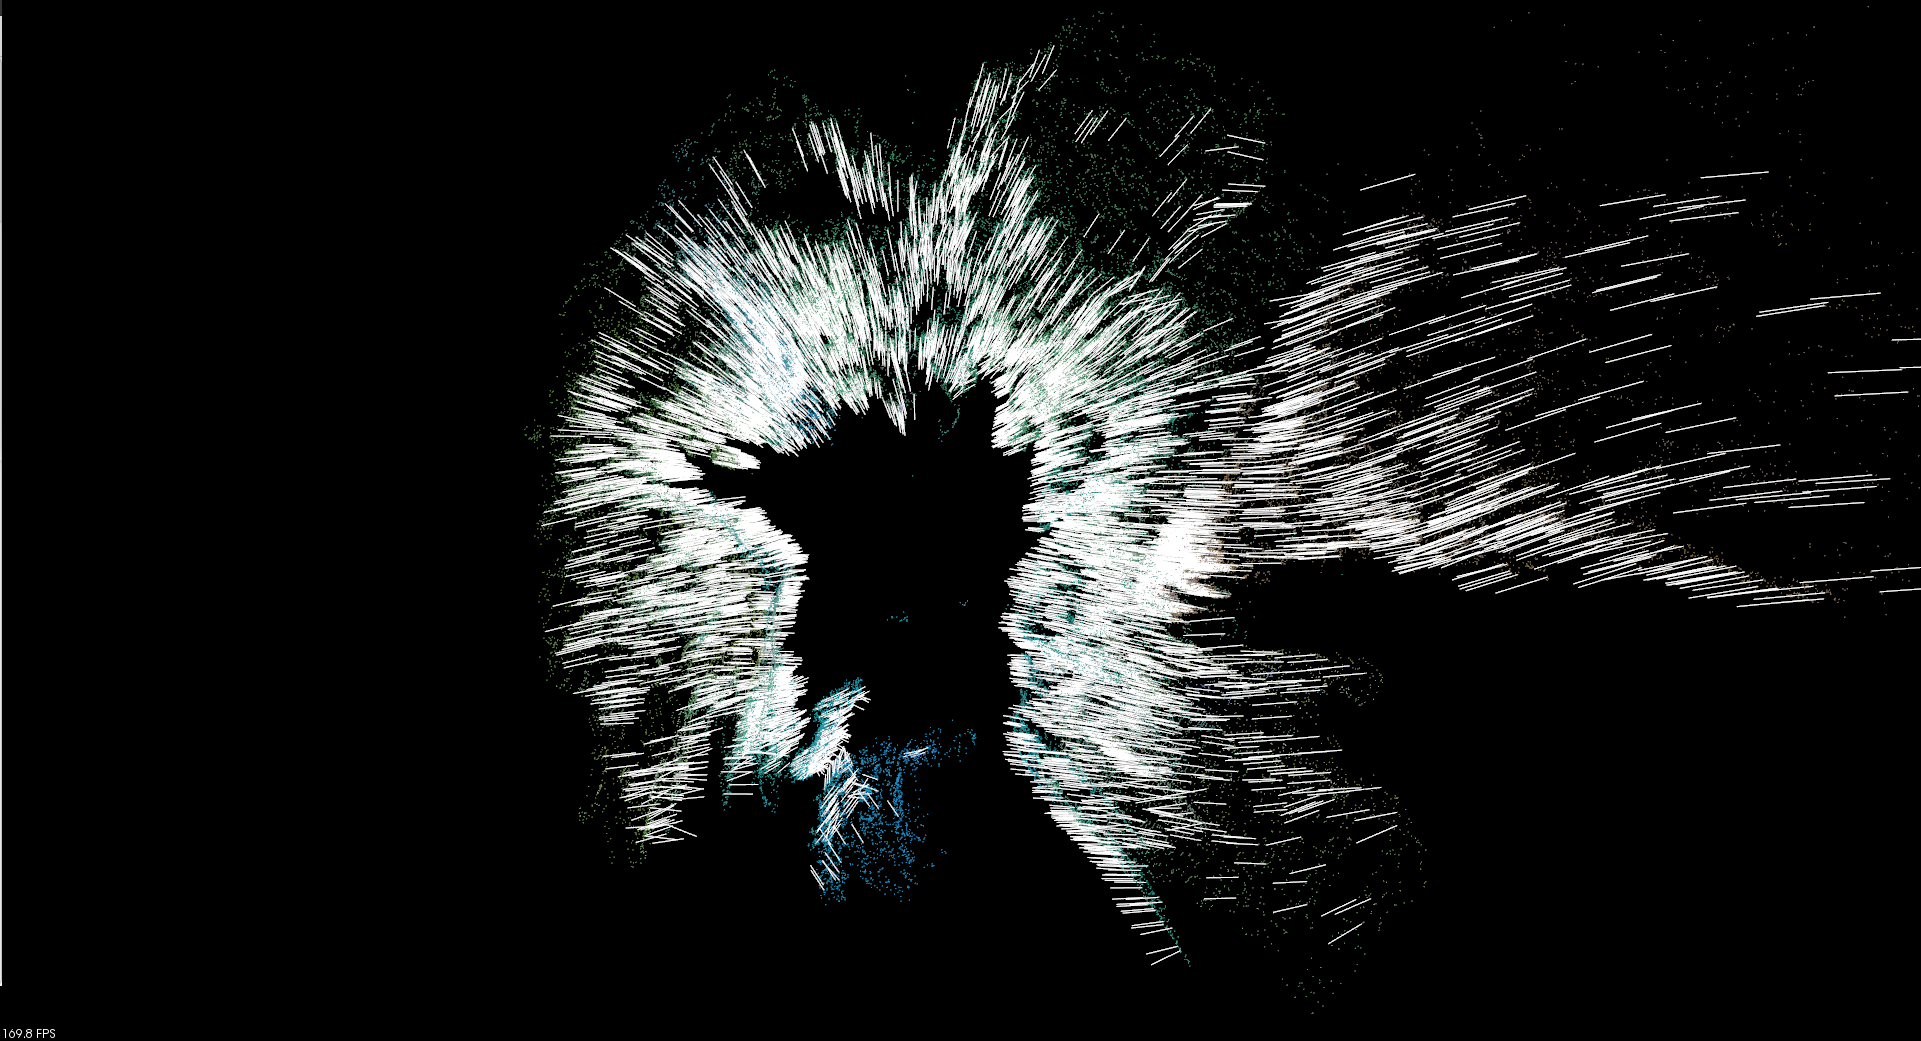
\includegraphics[width=0.95\textwidth]{./figures/normals_pcl_with}\label{fig:with_normals}}}
		\end{tabular}
		\caption{\ref{fig:without_normals} A point cloud segment of the ten second traversal. \ref{fig:with_normals} The same segment with white normal lines protruding inwards}
		\label{fig:showing_normals}
	\end{center}
\end{figure*}

Moving this normal oriented point cloud over to Meshlab allows us to now experiment with the different reconstruction techniques. These tests were run on the points generated from the first 100 frames of the ten second traversal video. Ultimately our reconstruction would never run on the full frame data set due to processing power constraints, so instead the cave would be generated in subsets and stitched together. 100 frames was enough to define the shape of the walls, and adding in more had minimal effect on the local outputs. Textures were generated using the RGB values of the input points. This looses a lot of the texture detail present in the images themselves, but a base model needed to be established first before creating a proper texture projection.  

An initial test was done using only Delaunay triangulation. This was the procedure that had been used on ocean floor mosaicking were the overall shape of the points was flatter. Unfortunately for our point cloud, Delaunay triangulation creates a completely incomprehensible mass. 

\begin{figure}[h]
	\centering
	\fbox{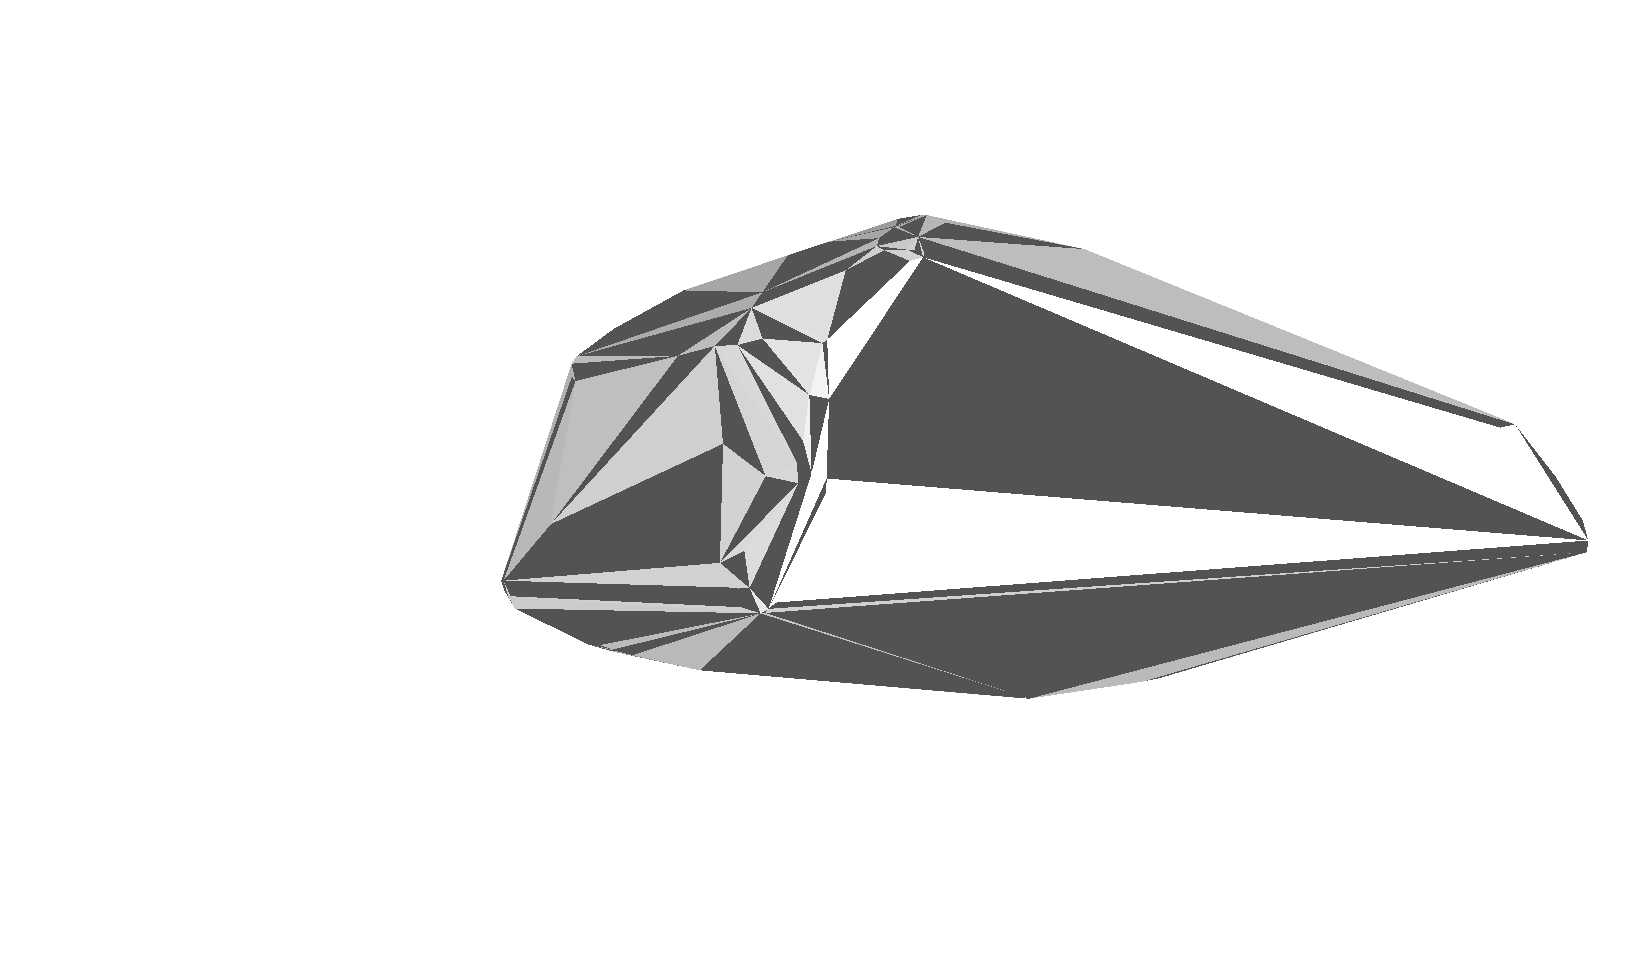
\includegraphics[width=0.95\columnwidth]{./figures/deltri01}}
	\caption{Results of running Delaunay triangulation.}
	\label{fig:deltri}
\end{figure}

\begin{figure*}[h]
	\begin{center}
		\leavevmode
		\begin{tabular}{ccc}
			\subfloat[]{\fbox{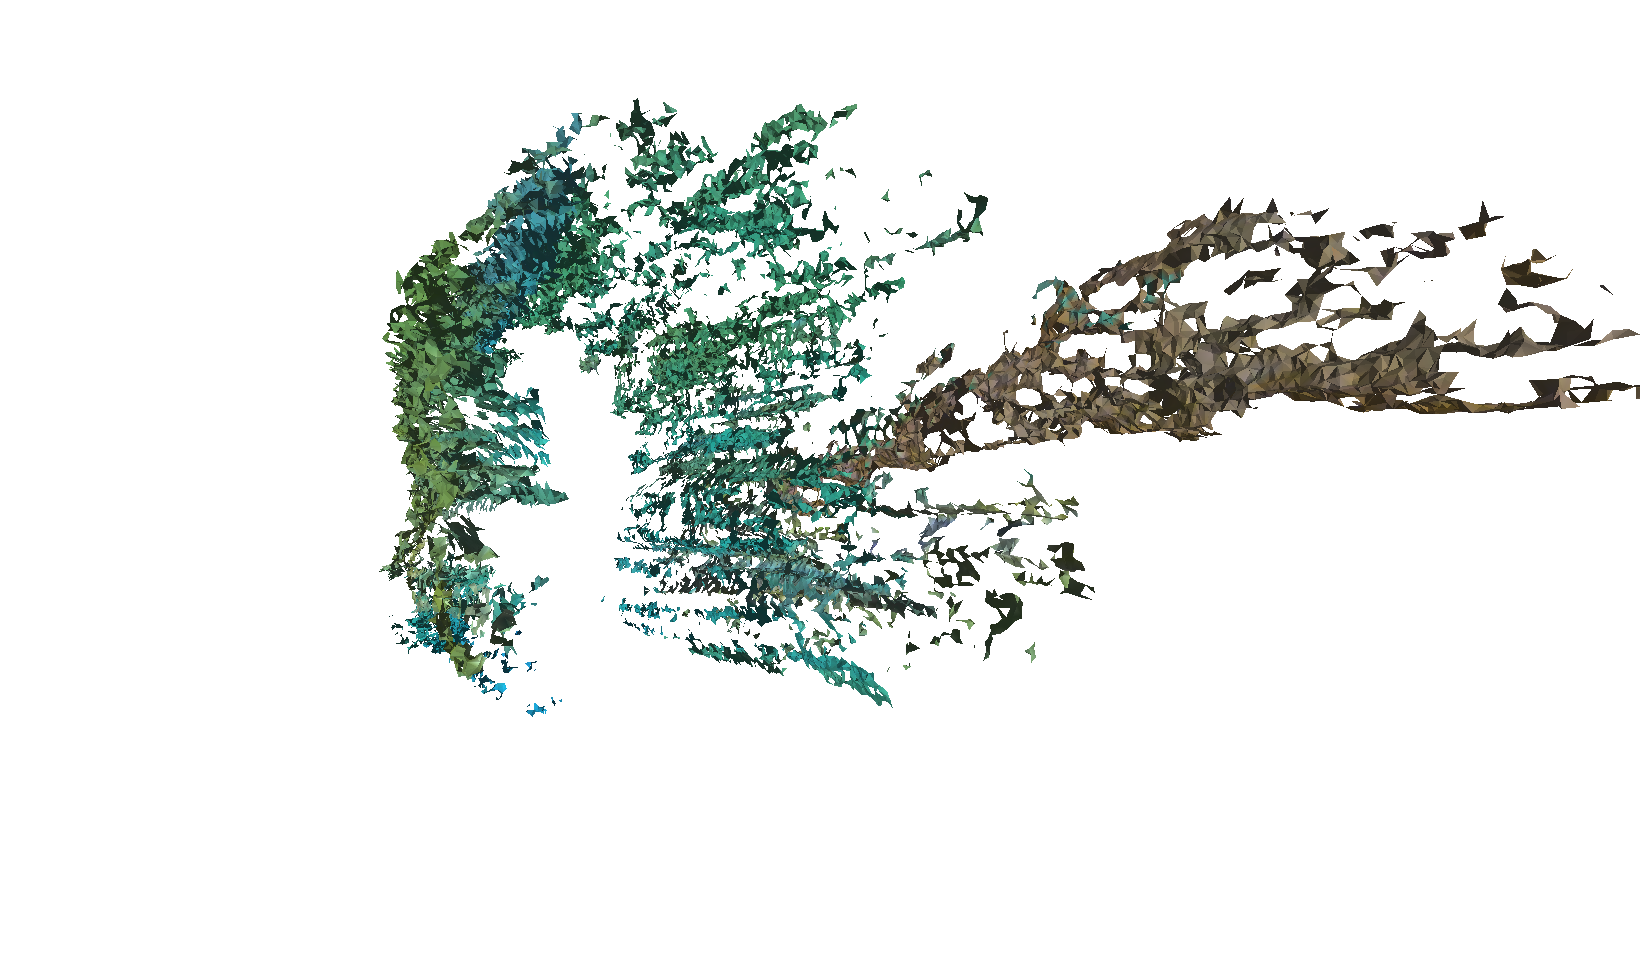
\includegraphics[width=0.55\textwidth]{figures/bp_all00}\label{fig:bp_all}}}\\
			\subfloat[]{\fbox{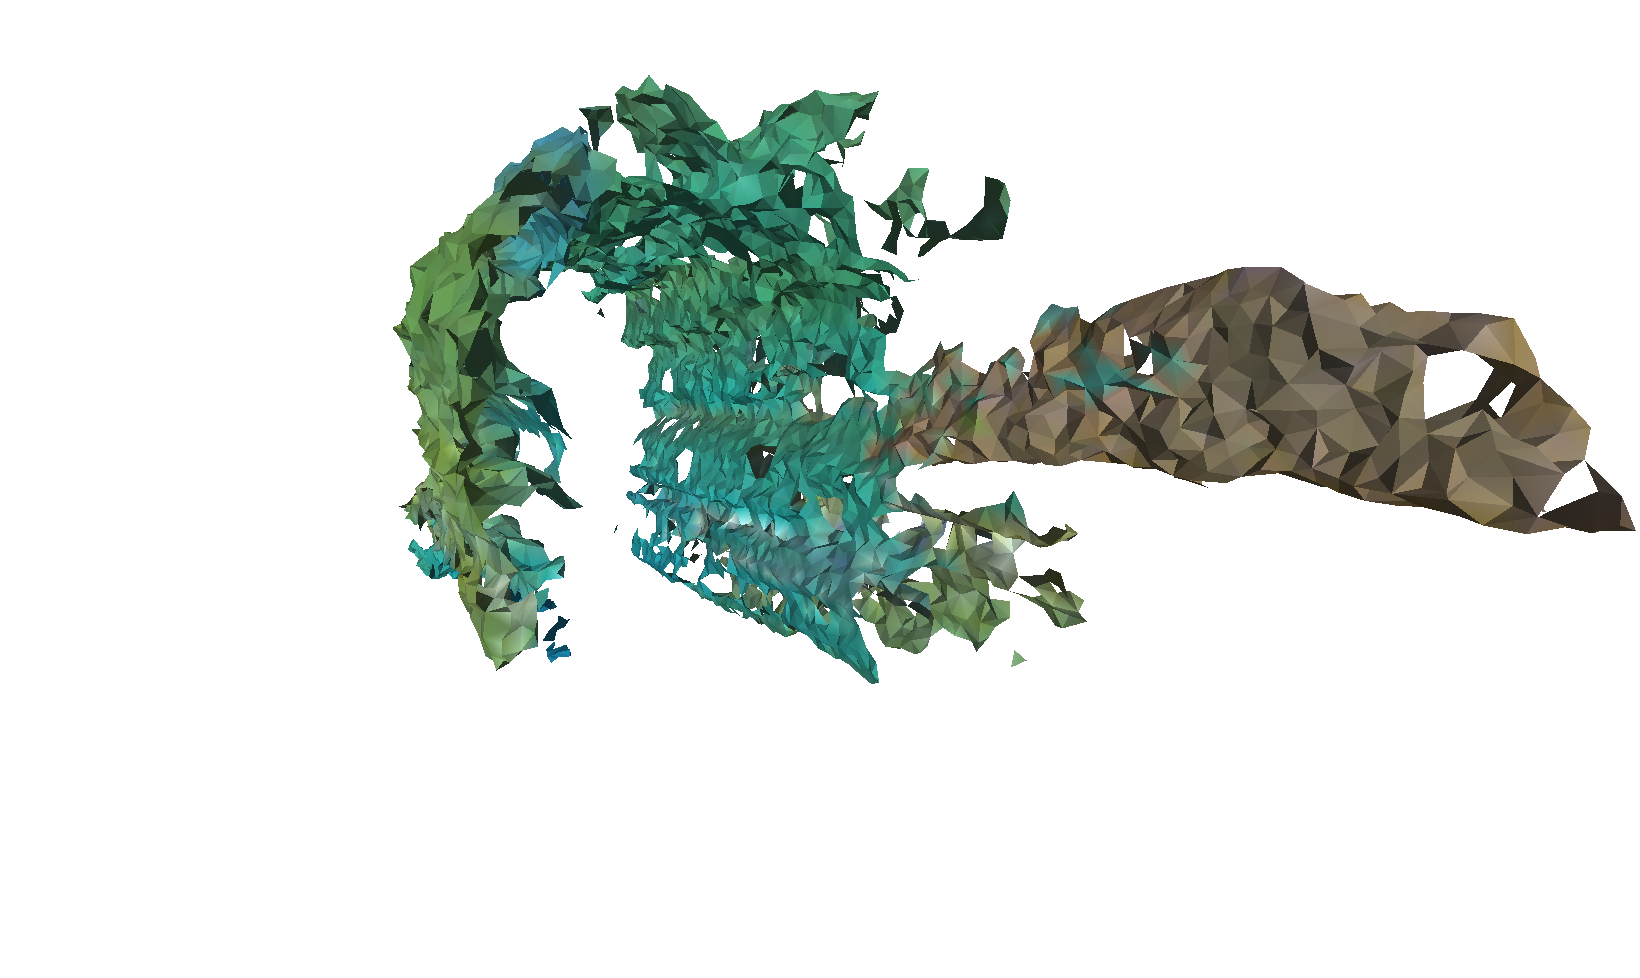
\includegraphics[width=0.55\textwidth]{figures/bp_tenthou00}\label{fig:bp_tenthou}}}\\
			\subfloat[]{\fbox{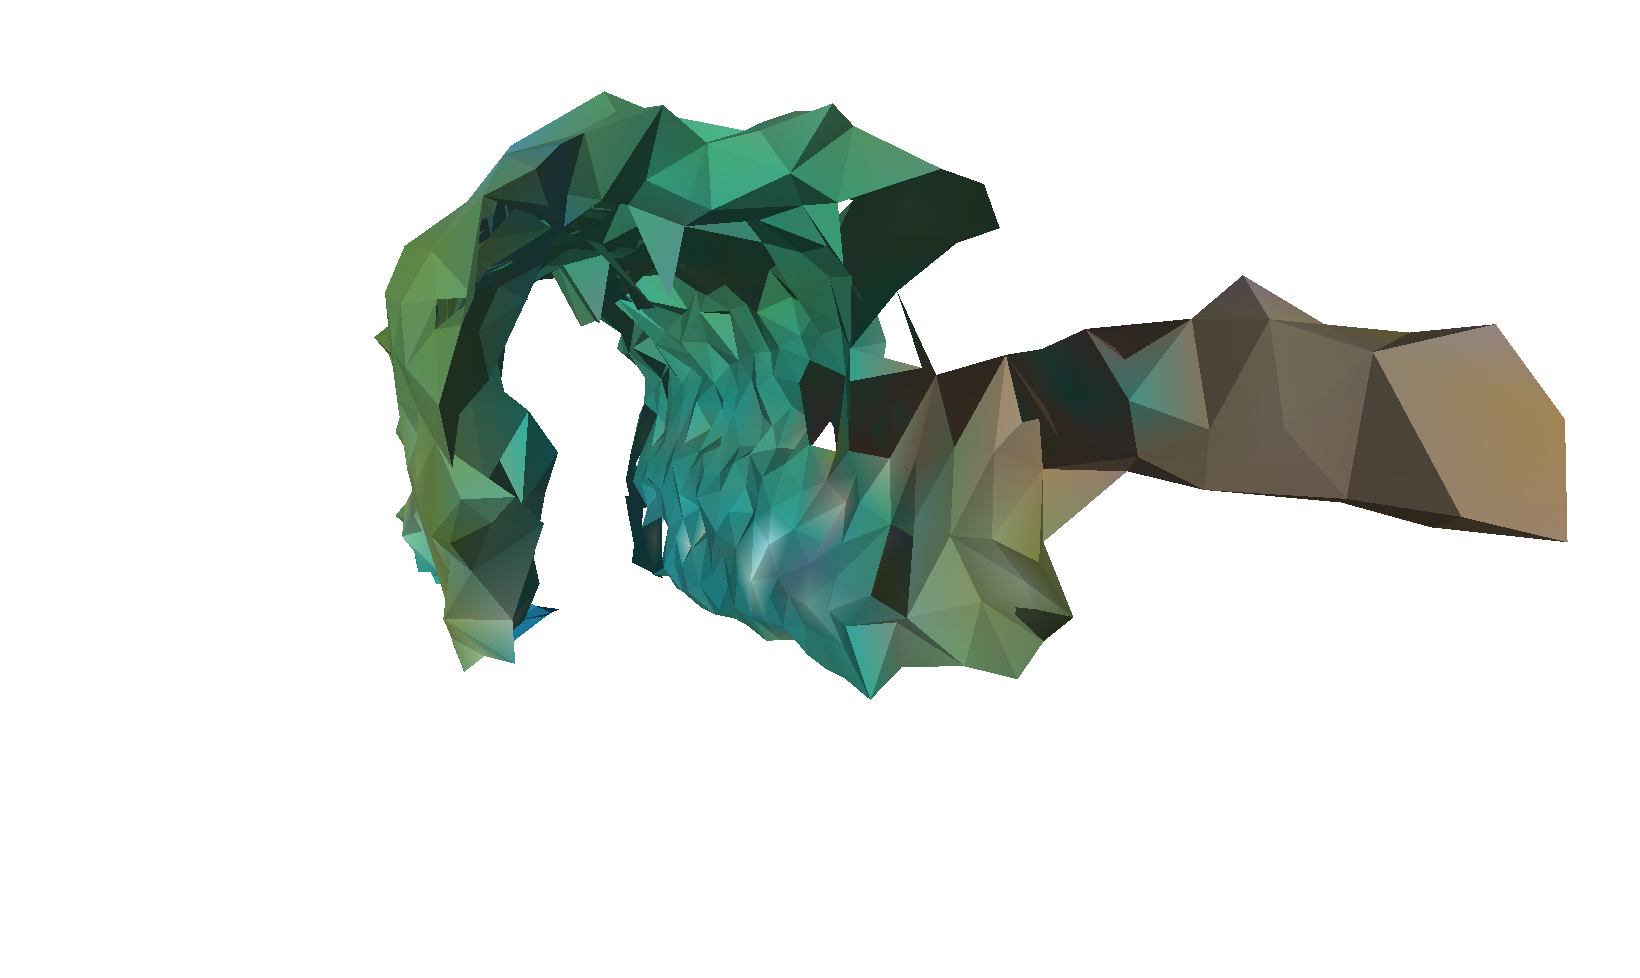
\includegraphics[width=0.55\textwidth]{figures/bp_thou01}\label{fig:bp_thou}}} 
		\end{tabular}
	\end{center}
	\caption{\ref{fig:bp_all} Ball-pivoting applied to the entire point set. \ref{fig:bp_tenthou} Applied to a 10,000 sampling. \ref{fig:bp_thou} Applied to 1,000 point sampling.}
	\label{fig:ballPivot}
\end{figure*}

If we try an interpolative method such as ball-pivoting, we see in \ref{fig:bp_all} that the results don't look much better than Delaunay triangulation. If we take sampling into account, though, dropping the total point count down from 100,000 points to 10,000 or 1,000 produces fast low res versions of the cave mesh as seen in \ref{fig:bp_tenthou} and \ref{fig:bp_thou} respectively. These can be useful in quickly generating surfaces that have at least some resemblance of the shape. 



Meshlab includes two marching-cubes based reconstruction approaches using MLS, algebraic point set surfaces (APSS)~\cite{guennebaud2007algebraic,guennebaud2008dynamic} and robust implicit MLS (RIMLS)~\cite{oztireli2009feature}. After adjusting the MLS filter scale, these methods generate the best reconstructions achieved. Both produce similar outputs, but the RIMLS method appears to create smoother surfaces in a more locations. These results are shown in \ref{fig:rimls}.

\begin{figure}[h]
	\centering
	\fbox{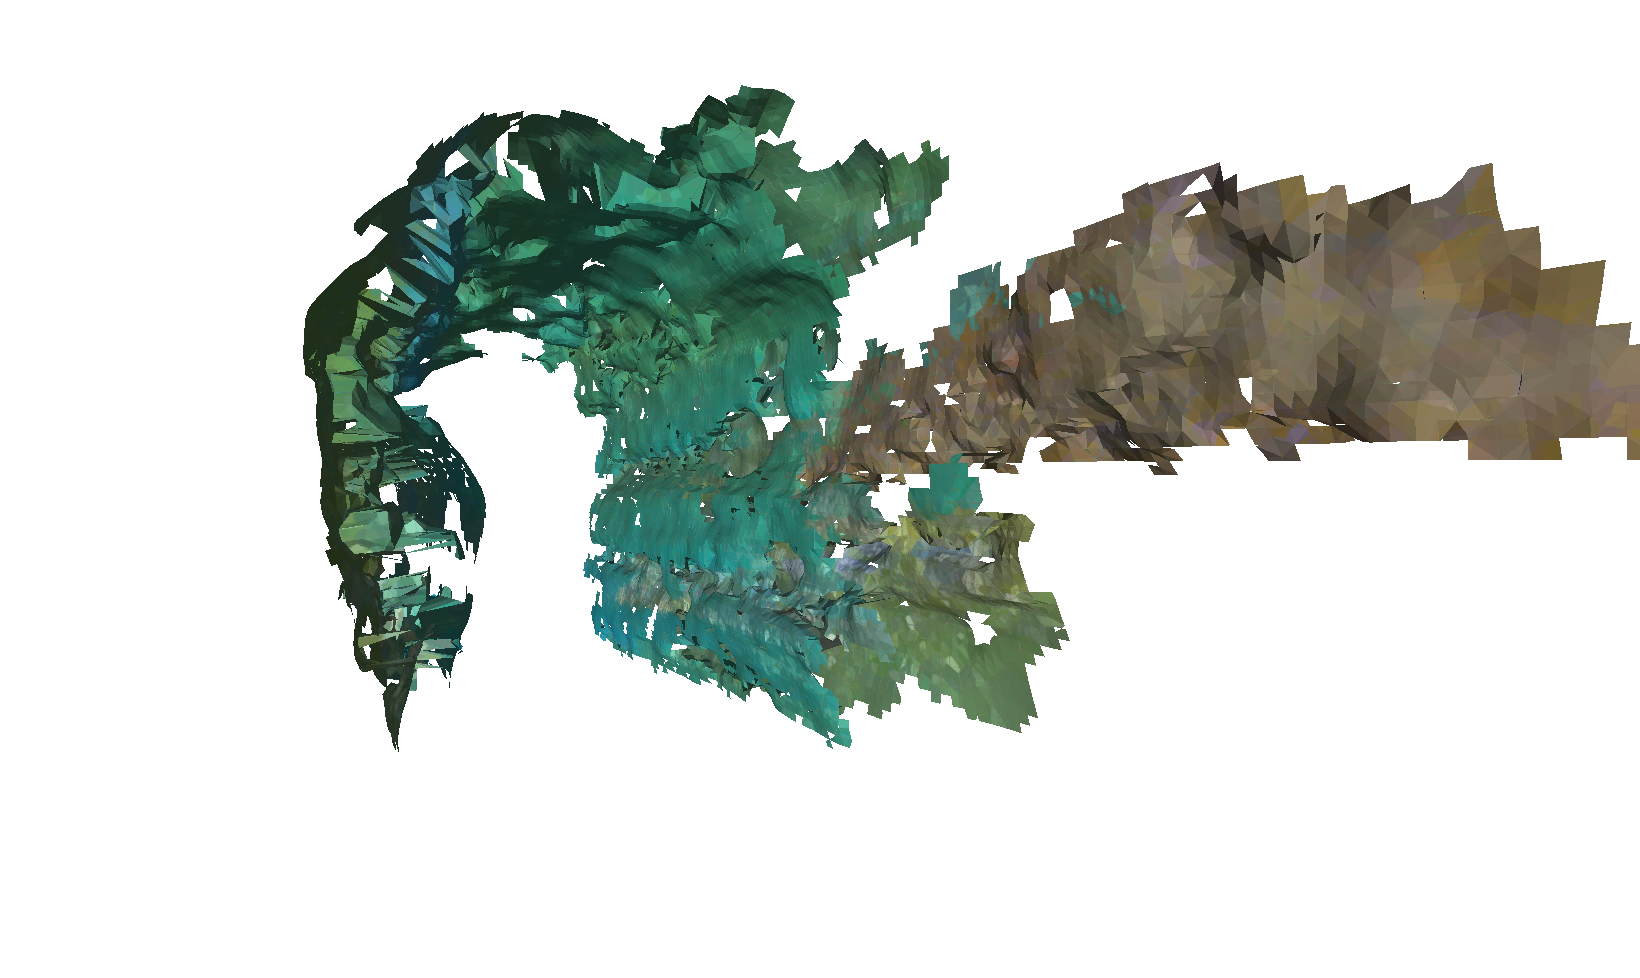
\includegraphics[width=0.95\columnwidth]{./figures/rimls00}}
	\caption{RIMLS marching cubes surface reconstruction}
	\label{fig:rimls}
\end{figure}

It is clear the shape of the cave is still not perfect. It is expected most of problems arise from our camera set up and lack of input data detail. Due to our small baseline, We loose a lot of accuracy as we move away from the camera. This is likely a cause for the misalignment occurring along the walls. These kinds of errors in our reprojection can cause reconstruction problems when points fall to closely to other points they shouldn't be near. Testing with other camera systems should shed light on areas of our reconstruction pipeline that can benefit from finer tuning. 